\begin{frame}{Operation system functions.}
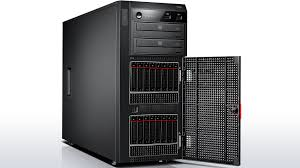
\includegraphics[height=2cm]{hw_tower.jpg} 
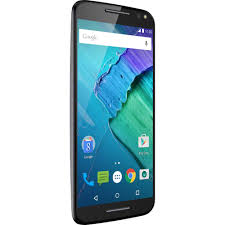
\includegraphics[height=2cm]{hw_smartphone.jpg}
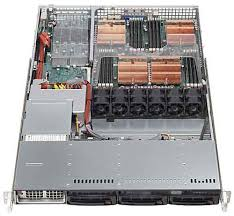
\includegraphics[height=2cm]{server_1u.jpg}
	\begin{itemize}
            \item Is it possible to work without OS?
            \item Why it is necessary?
	    \item What does OS do?
	\end{itemize}
\end{frame}

\begin{frame}{Operation system GNU/Linux components.}
    \begin{columns}
        \column{0.6\textwidth}
    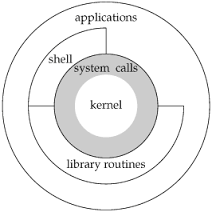
\includegraphics[scale=1]{unix_arch_highlevel}
        \column{0.4\textwidth}
	\begin{itemize}
		\item Kernel (Linux)
		\item Libraries (glibc)
                \item Compiler (GCC) 
		\item System utilities and applications (Userspace)
	\end{itemize}
    \end{columns}
\end{frame}
